\subsection{Recap: Object-Oriented Key Concepts}
\begin{frame}{\myframetitle}
	\leftorright{
		\mydefinition{Encapsulation}{Abstraction \& Information Hiding}		
		\mydefinition{Composition}{Nested objects}	
		\mydefinition{Message Passing}{Delegating responsibility}	
	}{
		\mydefinition{Distribution of Responsibility}{Separation of concerns}	
		\mydefinition{Inheritance}{Conceptual hierarchy, polymorphism, reuse}	
	}
\end{frame}

\subsection{Recap: Design Patterns}
\begin{frame}{\myframetitle\ \mytitlesource{\gof}}
	\leftorright{
		\vspace{-10mm}
		\mynote{Design patterns}{
			\begin{itemize}
				\item Document common solutions to concrete yet frequently occurring design problems.
				\item Suggest a concrete implementation for a specific object-oriented programming problem.
			\end{itemize}
		}		
		\mynote{Design patterns for variability}{
			\begin{itemize}
				\item Many GoF design patterns for designing software around stable abstractions and interchangeable (i.e., variable) parts, e.g.
				\begin{itemize}
					\item Template Method
					\item Abstract Factory
					\item Decorator
				\end{itemize}
			\end{itemize}
		}				
	}{
		\pic[width=\linewidth]{gof}
	}
\end{frame}

\subsection{Template Method Pattern}
\begin{frame}{\myframetitle}
	\leftorright{
		\mydefinition{Template Method \mysource{\gof}}{
			\begin{itemize}
				\item {\bf Intent:} \mycite{Define the overall structure of an algorithm, while allowing subclasses to refine, or redefine, certain steps.}
				\item {\bf Motivation:}  Avoid code replication by implementing the general workflow of an algorithm once, while allowing for necessary variations.
				\item {\bf Idea:} A template method defines the skeleton of an algorithm. Concrete methods override the hook methods.
			\end{itemize}
		}{}
	}{
		\pic[width=\linewidth]{templatemethod}
	}
\end{frame}

\subsection{Abstract Factory Pattern}
\begin{frame}{\myframetitle}
	\leftorright{
		\mydefinition{Abstract Factory \mysource{\gof}}{
			\begin{itemize}
				\item {\bf Intent:} \mycite{Provide an interface for creating families of related or dependent objects without specifying their concrete classes.}
				\item {\bf Motivation:} Avoid case distinctions when creating objects of certain kind, consistently create objects of a particular kind.
				\item {\bf Idea:} Create classes for the consistent creation of objects.
			\end{itemize}
		}{}
	}{
		\pic[width=\linewidth]{abstractfactory}
	}
\end{frame}

\subsection{Decorator Pattern}
\begin{frame}{\myframetitle}
	\leftorright{
		\mydefinition{Decorator \mysource{\gof}}{
			\begin{itemize}
				\item {\bf Intent:} \mycite{Attach additional responsibilities to an object dynamically. Decorators provide a flexible alternative to subclassing for extending functionality.}
				\item {\bf Motivation:} Avoid explosion of static classes when combining all additional behaviors with all applicable classes.
				\item {\bf Idea:} Create decorators and components with the same interface, whereas decorators forward behavior whenever feasible.
			\end{itemize}
		}
	}{
		\pic[width=\linewidth]{decorator}
	}
\end{frame}

\subsection{Object-Oriented Design of our Graph Library}
\begin{frame}{\myframetitle}
	\leftorright{
		\begin{center}
			\pic[width=0.7\linewidth]{graphlib-oo-node-edge}
		\end{center}
	}{
		\pic[width=\linewidth]{graphlib-oo-graph}
	}
\end{frame}

\begin{frame}[fragile]{Instantiation through Template Method Pattern}
		\begin{columns}
			\column{.45\textwidth}
\begin{tiny}
\begin{lstlisting}
public class Graph {
	...
	Edge add(Node n, Node m) {
		Edge e = createEdge();
		nv.add(n); nv.add(m); ev.add(e);
		return e;
	}
	
	// hook method (with default implementation)
	Edge createEdge(Node n, Node m) {
		return new Edge(n, m);
	}
	...
}
\end{lstlisting}
\begin{lstlisting}
@public class WeightedGraph extends Graph {
	...
	// override hook method
	Edge createEdge(Node n, Node m) {
		Edge e = new WeightedEdge(n, m);
		e.weight = new Weight();
		return e;
	}
	...
}@
\end{lstlisting}
\end{tiny}	
			\column{.45\textwidth}
				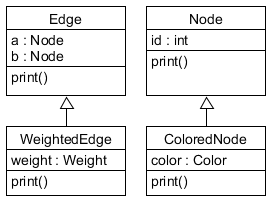
\includegraphics[width=0.75\linewidth]{graphlib-oo-node-edge}	
		\end{columns}
\end{frame}

\begin{frame}[fragile]{Instantiation through Abstract Factory Pattern}
		\begin{columns}
			\column{.45\textwidth}
\begin{tiny}
\begin{lstlisting}
public class Graph implements IGraph {
	EdgeFactory ef;
	...
	public Graph(EdgeFactory _ef) {
		ef = _ef;
	}
	
	public Edge add(Node n, Node m) {
		Edge e = ef.createEdge(n, m);
		nodes.add(n); nodes.add(m); edges.add(e);
		return e;
	}
	...
}
\end{lstlisting}
\begin{lstlisting}
public class EdgeFactory {
	Edge createEdge(Node a, Node b) {
		return new Edge(a, b);
	}
}
\end{lstlisting}
\begin{lstlisting}
@public class WeightedEdgeFactory extends EdgeFactory {
	Edge createEdge(Node a, Node b) {
		return new WeightedEdge(a, b);
	}
}@
\end{lstlisting}
\end{tiny}	
			\column{.45\textwidth}
				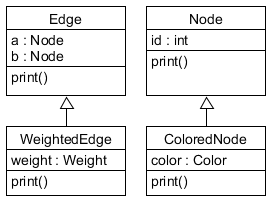
\includegraphics[width=0.75\linewidth]{graphlib-oo-node-edge}	
		\end{columns}
\end{frame}

\subsection{Feature Combinations}
\begin{frame}{Feature Combinations?}
	\leftorright{
		\begin{center}
			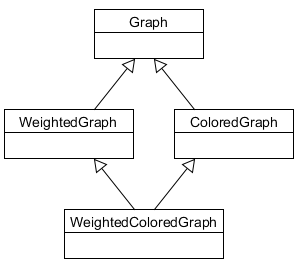
\includegraphics[width=\linewidth]{graphlib-oo-diamond}
		\end{center}		
	}{
	}
\end{frame}

\begin{frame}{Diamond Problem}
	\leftorright{
		\mynote{Multiple Inheritance}{
			\begin{itemize}
				\item Remember that most object-oriented programming languages do not support multiple inheritance (or only provide workarounds).
			\end{itemize}
		}
	}{
		\begin{center}
			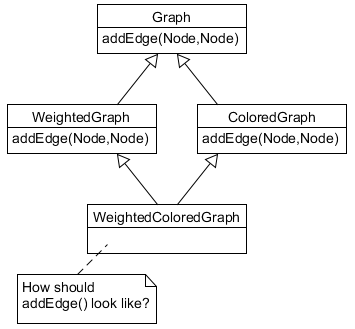
\includegraphics[width=\linewidth]{graphlib-oo-diamond-commented}
		\end{center}		
	}
\end{frame}

\begin{frame}{Static Modeling of Feature Combinations}
	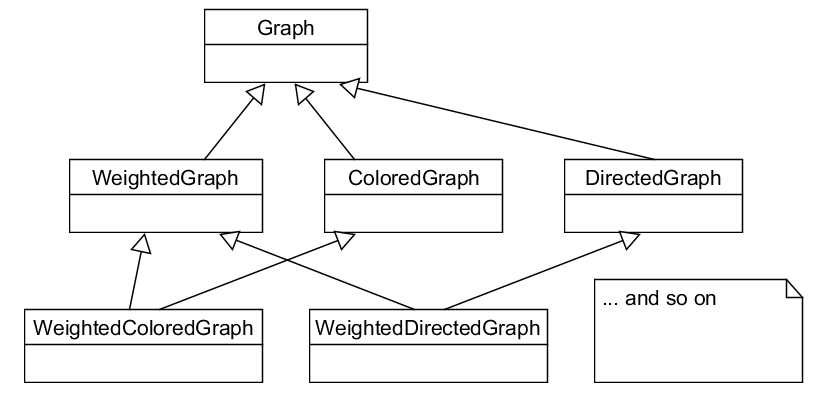
\includegraphics[width=0.7\linewidth]{graphlib-oo-combinatorial}
	\mynote{}{
		Even if multiple inheritance is supported, statically combining features through inheritance is tedious (or infeasible).
	}
\end{frame}

\begin{frame}[fragile]{Decorator Pattern as a Solution?}
		\begin{columns}
			\column{.45\textwidth}
\begin{tiny}
\begin{lstlisting}
public abstract class GraphDecorator implements IGraph {
	protected IGraph graph;
	
	public GraphDecorator(IGraph _graph) { 
		graph = _graph; 
	}
}
\end{lstlisting}
\begin{lstlisting}
@public class WeightedGraph extends GraphDecorator {
	public WeightedGraph(IGraph _graph) {
		super(_graph);
	}
	public Edge add(Node n, Node m) {
		WeightedEdge e = (WeightedEdge) graph.add(n, m);
		e.weight = new Weight();
		return e;
	}
	...
}@
\end{lstlisting}
\end{tiny}	
			\column{.45\textwidth}
				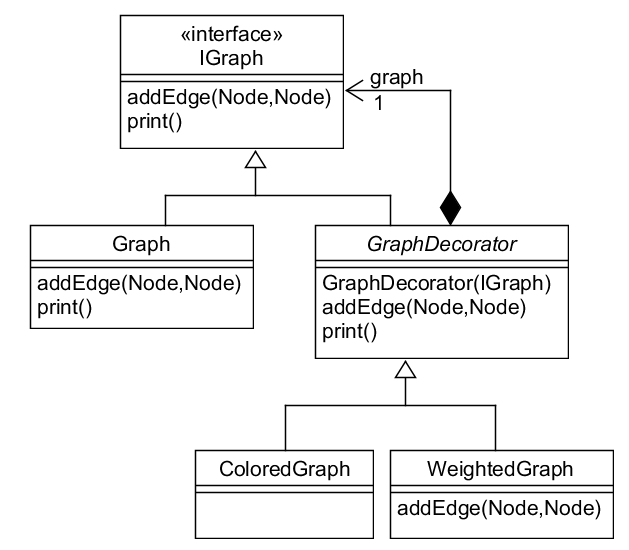
\includegraphics[width=\linewidth]{graphlib-oo-decorator}	
		\end{columns}
Usage Example: 
\begin{tiny}
\begin{lstlisting}
IGraph g = new WeightedGraph(new ColoredGraph(new Graph(new WeightedEdgeFactory())));
\end{lstlisting}
\end{tiny}	
\end{frame}

\begin{frame}{Delegation instead of Inheritance}
	\leftorright{
		\mynote{Discussion}{
			Extensions (i.e., features) can be combined dynamically, but \ldots
			\begin{itemize}
				\item \ldots must be independent of each other,
				\item \ldots cannot add public methods,
				\item \ldots plenty of indirections,
				\item \ldots several physical objects are forming a conceptual one.
			\end{itemize}
		}
	}{
		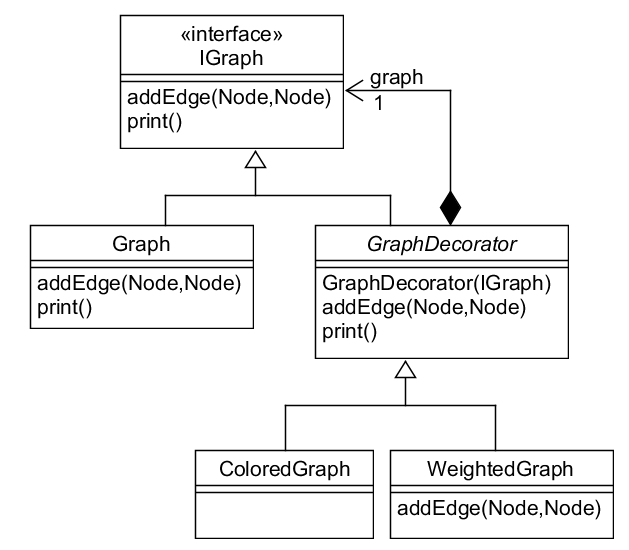
\includegraphics[width=\linewidth]{graphlib-oo-decorator}
	}
\end{frame}